\documentclass[a4paper,12pt]{article}
\usepackage{HomeWorkTemplate}
\usepackage{circuitikz}
\usepackage[shortlabels]{enumitem}
\usepackage{float}
\usepackage{hyperref}
\usepackage{tikz}
\usepackage{amsmath}
\usepackage{amssymb}
\usepackage{tcolorbox}
\usepackage{xepersian}
\settextfont{XB Niloofar}
\usetikzlibrary{arrows,automata}
\usetikzlibrary{circuits.logic.US}
\usepackage{changepage}
\newcounter{problemcounter}
\newcounter{subproblemcounter}
\setcounter{problemcounter}{1}
\setcounter{subproblemcounter}{1}
\newcommand{\problem}[1]
{
	\subsection*{
		پرسش
		\arabic{problemcounter} 
		\stepcounter{problemcounter}
		\setcounter{subproblemcounter}{1}
		#1
	}
}
\newcommand{\subproblem}{
	\textbf{\harfi{subproblemcounter})}\stepcounter{subproblemcounter}
}


\begin{document}
\handout
{آز طراحی سیستم‌های دیجیتال}
{دکتر سیاوش بیات سرمدی}
{نیم‌سال اول 1400\lr{-}1401}
{اطلاعیه}
{ \newline حسین آقایی \newline پرهام چاوشیان}
{\newline 98105619 \newline 98100118 }
 {گزارش آزمایش هفتم}
 {خانم زینب رشیدی}
دو ماژول
$sender$
و
$reciever$
داریم که به ترتیب نام آن‌ها
$UART$
و
$reciever$
است.\\
در ماژول $sender$ زمانی که فرمان شروع بیاید به حالت $START$ می‌رویم و بیت خروجی 1 می‌شود. بعد از آن بیت $PARITY$ فرستاده می‌شود و سپس بیت‌ها داده فرستاده می‌شوند و در نهایت هم بیت $STOP$ فرستاده می‌شود.\\
در ماژول $reciever$ بیت‌هایی که ماژول $sender$ می‌فرستد را به ترتیب دریافت می‌کنیم. در نهایت زوجیت بیت‌های داده شده را با زوجیت اعلام شده چک می‌کنیم.
نتایج شبیه‌سازی نیز در ادامه آمده است، دقت کنید که خروجی تنها در پالس ساعتی که خروجی $done$ برابر 1 شده است، معتبر است. (در صورت نیاز تصاویر به طور جداگانه نیز پیوست شده اند):
\begin{figure}[H]
 \centering
  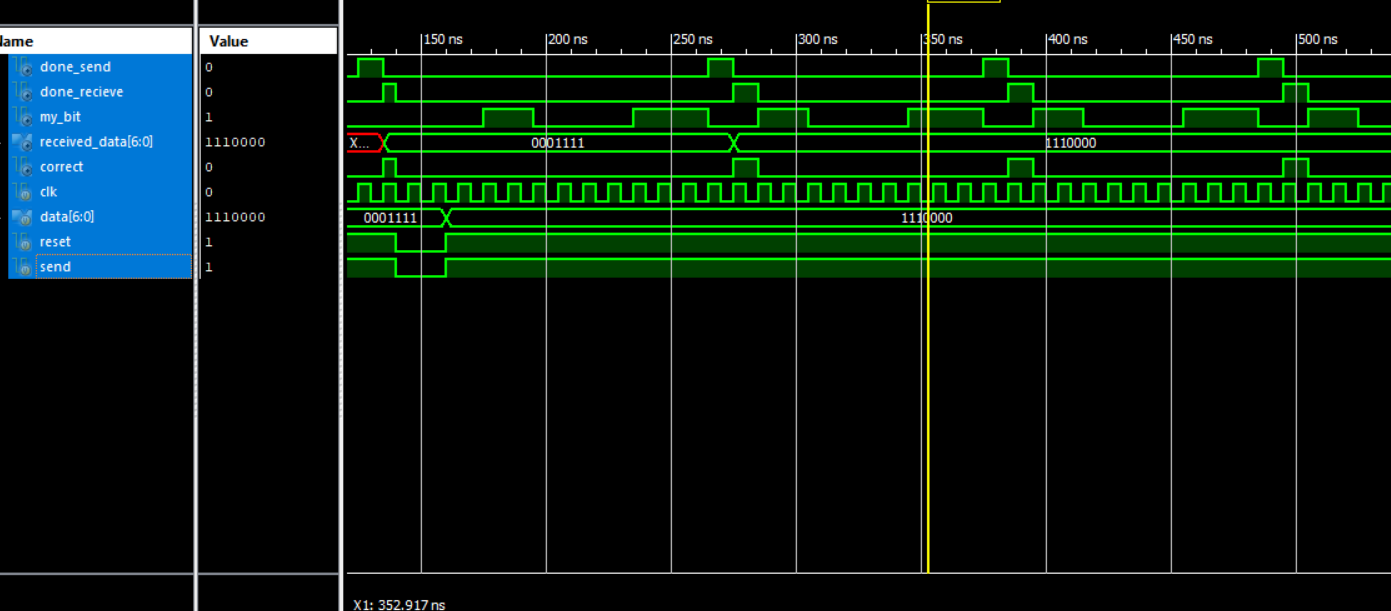
\includegraphics[width=0.8\linewidth]{s1}
\end{figure}
\end{document}
